% Created 2023-10-22 Sun 16:57
% Intended LaTeX compiler: pdflatex
\documentclass[11pt]{article}
\usepackage[utf8]{inputenc}
\usepackage[T1]{fontenc}
\usepackage{graphicx}
\usepackage{longtable}
\usepackage{wrapfig}
\usepackage{rotating}
\usepackage[normalem]{ulem}
\usepackage{amsmath}
\usepackage{amssymb}
\usepackage{capt-of}
\usepackage{hyperref}
\usepackage{siunitx, graphicx}
\graphicspath{ {./images/} }
\author{Hankertrix}
\date{\today}
\title{Physics Electric Fields Cheat Sheet}
\hypersetup{
 pdfauthor={Hankertrix},
 pdftitle={Physics Electric Fields Cheat Sheet},
 pdfkeywords={},
 pdfsubject={},
 pdfcreator={Emacs 29.1 (Org mode 9.6.6)}, 
 pdflang={English}}
\begin{document}

\maketitle
\setcounter{tocdepth}{2}
\tableofcontents

\newpage

\section{Definitions}
\label{sec:org96c337a}

\subsection{Principle of charge conservation}
\label{sec:org33cc66f}
The principle of charge conservation states that the algebraic sum of all the electric charges in any closed system is constant.

\subsection{Coulomb's law}
\label{sec:org4706cd0}
Coulomb's law states that the force between two \textbf{point charges} is given by:
\[F = \frac{1}{4 \pi \varepsilon_0} \frac{q_1 q_2}{r^2}\]

Where:
\begin{itemize}
\item \(\varepsilon_0\) is the permittivity of vacuum, with a value of approximately \(\\ 8.85 \times 10^{-12} \ \unit{F.m^{-1}}\).
\item \(q_1\) is the charge of the first point charge.
\item \(q_2\) is the charge of the second point charge.
\end{itemize}

If the charges reside within a medium which contains atoms and molecules, like air, then the interaction of the medium with the charge will cause the effective force to be \textbf{reduced} by a factor \(\varepsilon_r = \frac{\varepsilon_{media}}{\varepsilon_0}\), which is called the relative permittivity of the medium. It is given by the ratio of the (absolute) permittivity of the medium to the vacuum permittivity of the medium to the vacuum permittivity, i.e. the force becomes:
\[F = \frac{1}{4 \pi \varepsilon_r \varepsilon_0} \frac{q_1 q_2}{r^2}\]

\newpage

\subsection{Principle of linear superposition}
\label{sec:orgc84578d}
The principle of linear superposition states that every charge in space creates an electric field at point \(\boldsymbol{r}\) independent of the presence of other charges in that medium. The resultant electric field is a vector sum of the electric field due to individual charges.

\subsubsection{Discrete charge distribution}
\label{sec:org751acb0}
\begin{align*}
\vec{E}_{net} (\vec{r}) &= \sum_{i} \vec{E}_{i} (\vec{r}) \\
&= \sum_{i} \frac{q_i}{4 \pi \varepsilon_0 |\vec{r} - \vec{r}_i|^2}
\end{align*}

\subsubsection{Continuous charge distribution}
\label{sec:org0a2ddf2}
\begin{align*}
\vec{E}_{net} (\vec{r}) &= \int \, d \vec{E} (\vec{r}) \\
&= \int \frac{1}{4 \pi \varepsilon_0 |\vec{r} - \vec{r}_i|^2} \, dq \\
&= \int \frac{\rho (\vec{r'})}{4 \pi \varepsilon_0 |\vec{r} - \vec{r}_i|^2} \, dV \\
\end{align*}

\newpage

\subsection{Electric dipole}
\label{sec:orgd83c7d5}
An electric dipole is an arrangement of two point charges, separated by a distance \(d\).
\\[0pt]

Even though an electric dipole is electrically neutral, it interacts with an external electric field. An electric dipole \textbf{experiences torque in a uniform electric field}.
\[\vec{\tau} = \vec{p} \times \vec{E} \]

Where:
\begin{itemize}
\item \(\vec{\tau}\) is the torque vector on an electric dipole
\item \(\vec{p}\) is the electric dipole moment
\item \(\vec{E}\) is the electric field
\end{itemize}

This torque causes the dipole to undergo rotation or angular displacement, which means that there is work done by the electric field on the dipole.
\\[0pt]

A net force can only experienced by a dipole placed in a \textbf{non-uniform} electric field.

\subsection{Dipole moment (SI Unit: \(\unit{C.m}\))}
\label{sec:orgcd810b4}
The dipole moment, \(p\) is a \textbf{vector} which points from the \textbf{negative to the positive} point charge.
\[p = qd\]

\subsection{Electric potential}
\label{sec:org4831999}
Electric potential is defined as the potential energy per unit charge.
\[V = \frac{U}{q}\]

Where:
\begin{itemize}
\item \(V\) is the electric potential
\item \(U\) is the electric potential energy
\item \(q\) is the electric charge
\end{itemize}

Electric potential is also the \textbf{negative} of the integral of the electric field:
\[V = - \int \vec{E} \, d \vec{r}\]

\subsubsection{Single point charge}
\label{sec:orgac85d22}
\[V = \frac{1}{4 \pi \varepsilon_0} \frac{q}{r}\]

Where:
\begin{itemize}
\item \(V\) is the electric potential due to a point charge
\item \(\varepsilon_0\) is the permittivity of vacuum
\item \(q\) is the value of the point charge
\item \(r\) is the distance from the point charge to where the potential is measured
\end{itemize}

\subsubsection{Collection of point charges}
\label{sec:org727a8a8}
\[V = \frac{1}{4 \pi \varepsilon_0} \sum_i \frac{q_i}{r_i}\]

Where:
\begin{itemize}
\item \(V\) is the electric potential due to a collection of point charges
\item \(\varepsilon_0\) is the permittivity of vacuum
\item \(q\) is the value of the \(i^{th}\) point charge
\item \(r_i\) is the distance from the \(i^{th}\) point charge to where the potential is measured
\end{itemize}

\subsubsection{Relationship with electric field}
\label{sec:org6aaa5de}
Moving \textbf{with the direction of the electric field} means moving in the direction of \textbf{decreasing} potential and vice versa.

\newpage

\subsection{Potential difference}
\label{sec:org6236f3c}
The potential difference between two points is equal to the work done per unit charge by an external force in moving a test charge from one point to another.
\[V_{ba} = V_{b} - V_{a}\]

Where:
\begin{itemize}
\item \(a\) and \(b\) are two points in space
\item \(V\) is the electric potential
\item \(V_{ba}\) is the potential difference between points \(a\) and \(b\)
\end{itemize}

\subsubsection{In terms of electric field}
\label{sec:org44ec8ed}
\[V_{ba} = - \int_a^b \vec{E} \cdot d \vec{l}\]

Where:
\begin{itemize}
\item \(a\) and \(b\) are two points in space
\item \(V_{ba}\) is the potential difference between points \(a\) and \(b\)
\item \(\vec{E}\) is the electric field vector
\item \(d \vec{l}\) is the distance between points \(a\) and \(b\)
\end{itemize}

\subsection{Equipotential surfaces}
\label{sec:orgc3564f2}
An equipotential surface is a surface on which the electric potential is the same at every point. Field lines and equipotential surfaces are always perpendicular to each other.

\newpage

\section{Formulas}
\label{sec:org0babc58}

\subsection{Electric field of a point charge (SI Unit: \(\unit{N.C^{-1}} \text{ or } \unit{V.m^{-1}}\))}
\label{sec:org9601dc2}

\[\vec{E} = \frac{1}{4 \pi \varepsilon_0} \frac{q}{r^2} \hat{r}\]

Where:
\begin{itemize}
\item \(\vec{E}\) is the electric field due to a point charge.
\item \(\varepsilon_0\) is the permittivity of vacuum, with a value of approximately \(\\ 8.85 \times 10^{-12} \ \unit{F.m^{-1}}\).
\item \(q\) is the magnitude of the point charge.
\item \(r\) is the distance from the point charge to where the field is measured.
\item \(\hat{r}\) is the unit vector from the point charge towards where the field is measured.
\end{itemize}

\subsection{Electric field of a ring of charge}
\label{sec:org3d38aa6}
\[E = \frac{Q}{4 \pi \varepsilon_0} \frac{x}{(r^2 + x^2)^{\frac{3}{2}}}\]

Where:
\begin{itemize}
\item \(E\) is the magnitude of the electric field
\item \(Q\) is the total charge of the ring
\item \(\varepsilon_0\) is the permittivity of vacuum
\item \(r\) is the radius of the ring of charge
\item \(x\) is the distance away from the ring of charge
\end{itemize}

\newpage

\subsection{Electric field of a cylinder}
\label{sec:org095127e}
\[E = \frac{\lambda}{2 \pi \varepsilon_0 r}\]

Where:
\begin{itemize}
\item \(E\) is the magnitude of the electric field
\item \(\lambda\) is the charge per unit length
\item \(\varepsilon_0\) is the permittivity of vacuum
\item \(r\) is the radius of the cylinder
\end{itemize}

\subsection{Electric field of a long line of charge}
\label{sec:orgb7b067a}
\[E = \frac{1}{2 \pi \varepsilon_0} \frac{\lambda}{x}\]

Where:
\begin{itemize}
\item \(E\) is the magnitude of the electric field
\item \(\varepsilon_0\) is the permittivity of vacuum
\item \(\lambda\) is the charge per unit length (\(\unit{C.m^{-1}}\))
\item \(x\) is the distance from the long line of charge
\end{itemize}

\subsection{Electric field of an infinite thin plane of charge}
\label{sec:orgcd917f5}
\[E = \frac{\sigma}{2 \varepsilon_0}\]

Where:
\begin{itemize}
\item \(E\) is the magnitude of the electric field
\item \(\varepsilon_0\) is the permittivity of vacuum
\item \(\sigma\) is the uniform surface charge density (\(\unit{C.m^{-2}}\))
\end{itemize}

If there are 2 planes in the same direction, multiply the electric field by 2, i.e.
\[E = \frac{\sigma}{\varepsilon_0}\]

\subsection{Electric field at the surface of a conductor}
\label{sec:orge8c5509}
\[E_{\perp} = \frac{\sigma}{\varepsilon_0}\]

Where:
\begin{itemize}
\item \(E_{\perp}\) is the electric field at the surface of a conductor, which is also the \(\vec{E}\) perpendicular to the surface
\item \(\sigma\) is the surface charge density
\item \(\varepsilon_0\) is the permittivity of vacuum
\end{itemize}

This formula is very similar to the electric field for an infinite thin plane of charge, except that the electric field extends out from only \textbf{one side} and is \textbf{zero on the other side}. Thus, there is a difference by a factor of 2.

\subsection{Electric field in terms of electric potential}
\label{sec:orgc31b78e}
Each electric field component is equal to the \textbf{negative} of the corresponding partial derivative of the electric potential function \(V\).
\[\vec{E} = - \hat{x} \frac{\partial V}{\partial x} - \hat{y} \frac{\partial V}{\partial y} - \hat{z} \frac{\partial V}{\partial z} \equiv - \nabla V\]

\[E_x = - \frac{\partial V}{\partial x} \qquad E_y = - \frac{\partial V}{\partial y} \qquad E_z = - \frac{\partial V}{\partial z}\]

Where:
\begin{itemize}
\item \(E\) is the electric field components found from potential
\end{itemize}

In 2 dimensions, electric field is the \textbf{negative} of the differential of the electric potential:
\[E = -\frac{dV}{dr}\]

\subsubsection{Electric field between 2 uniformly charged plates}
\label{sec:orgd02e40e}
\[E = \frac{V}{d}\]

Where:
\begin{itemize}
\item \(E\) is the magnitude of the electric field
\item \(V\) is the potential difference between the two plates
\item \(d\) is the separation between the two plates
\end{itemize}

\newpage

\subsection{Electric flux (SI Unit: \(\unit{N.m^2.C^{-1}}\))}
\label{sec:org937d34a}
\begin{align*}
\Phi_E &= \int E \cos \phi \, dA \\
&= \int E_{\perp} \, dA \\
&= \int \vec{E} \cdot d \vec{A}
\end{align*}

Where:
\begin{itemize}
\item \(\Phi_E\) is the electric flux through a surface
\item \(E\) is the magnitude of the electric field
\item \(\phi\) is the angle between the electric field and the \textbf{normal to the surface}
\item \(dA\) is the element of surface area
\item \(E_{\perp}\) is the component of \(\vec{E}\) perpendicular to the surface
\item \(d \vec{A}\) is the vector element of the surface area
\end{itemize}

\subsection{Gauss' law}
\label{sec:org74474cb}
\begin{align*}
\Phi_E &= \oint \vec{E} \cdot d \vec{A} \\
&= \frac{Q_{encl}}{\varepsilon_0}
\end{align*}

Where:
\begin{itemize}
\item \(\Phi_E\) is the electric flux through a closed surface of area \(A\). It is equal to the surface integral of \(\vec{E}\).
\item \(Q_{encl}\) is the total charge enclosed by the surface
\item \(\varepsilon_0\) is the permittivity of vacuum
\end{itemize}

\subsection{Electric potential energy of 2 point charges}
\label{sec:org98eeca5}
\[U = \frac{1}{4 \pi \varepsilon_0} \frac{qq_0}{r}\]

Where:
\begin{itemize}
\item \(U\) is the electric potential energy of two point charges
\item \(\varepsilon_0\) is the permittivity of vacuum
\item \(q\) and \(q_0\) is the value of the two charges
\item \(r\) is the distance between the two charges
\end{itemize}

\subsection{Electric potential energy of a system of discrete charges}
\label{sec:orgdf88e6b}
\[U = \frac{1}{2} \sum_{i} \sum_{j \ne i} \frac{q_i q_j}{4 \pi \varepsilon_0 r_{ij}}\]

Where:
\begin{itemize}
\item \(U\) is the electric potential energy of two point charges
\item \(\varepsilon_0\) is the permittivity of vacuum
\item \(q_i\) and \(q_j\) is the value of the \(i^{th}\) and \(j^{th}\) charges
\item \(r\) is the distance between the \(i^{th}\) and \(j^{th}\) charges
\end{itemize}

We will have to consider \textbf{all pairwise interactions} for a system of discrete charges. The factor of \(\frac{1}{2}\) takes double counting into consideration.

\newpage

\subsection{Electric potential energy of a dipole's orientation in an electric field}
\label{sec:orge2fc372}
\begin{align*}
U &= - p E \cos \theta \\
&= - \vec{p} \cdot \vec{E}
\end{align*}

Where:
\begin{itemize}
\item \(U\) is the electric potential energy the dipole
\item \(\vec{p}\) is the electric dipole moment
\item \(p\) is the magnitude of the electric dipole moment
\item \(\vec{E}\) is the electric field
\item \(E\) is the magnitude of the electric field
\item \(\theta\) is the angle between the electric field and the dipole
\end{itemize}

\newpage

\section{Electric fields in conductors}
\label{sec:org3d410c8}
In conductors, there is:
\begin{itemize}
\item Zero electric field within the conductor
\item Zero tangential component of the electric field on the surface of the conductor
\end{itemize}

A charge inside a neutral spherical metal shell induces charge on its surfaces. The electric field exists even beyond the shell, but \textbf{not} within the conductor itself.
\[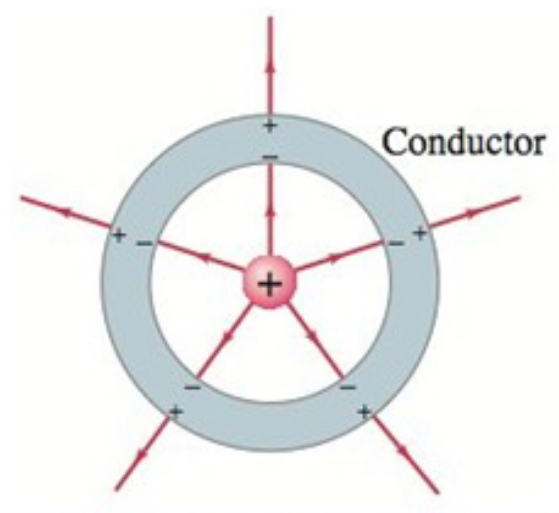
\includegraphics[scale = 0.65]{charge-inside-conductor}\]

For a conductor that \textbf{isn't moving}, the electric field parallel to the conductor \textbf{must be zero}, otherwise the conductor will \textbf{no longer be static}.
\\[0pt]

When all charges are at rest, the surface of a conductor is always an equipotential surface. The \textbf{electric field} just outside a conductor is always \textbf{perpendicular} to the surface.


\section{Summary of relationships}
\label{sec:org349bc37}
\[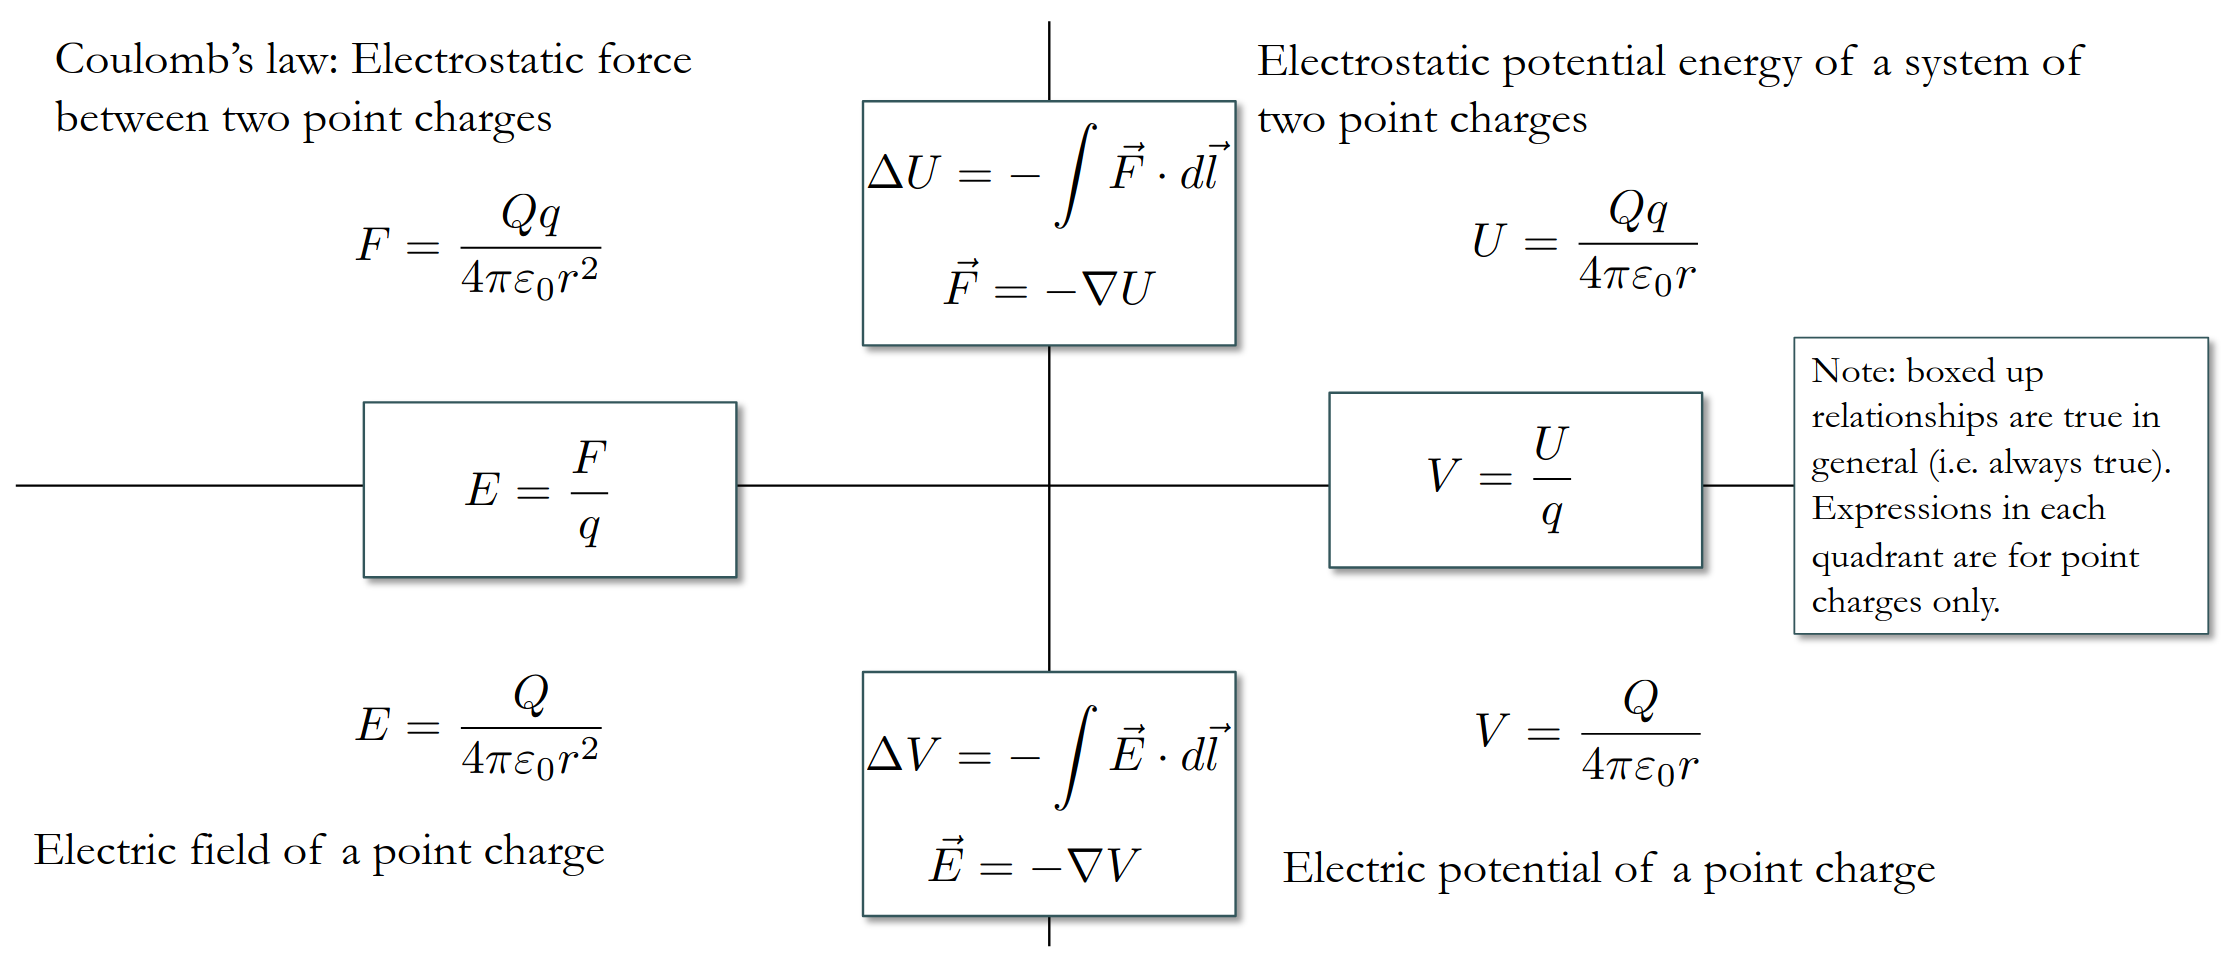
\includegraphics[width = \textwidth]{summary-of-relationships}\]
\end{document}